\chapter{Beeldvorming}
\section{Punten}
\begin{itemize}
	\item Elk 2D punt $(x, y)$ kan gerepresenteerd worden via de \textbf{homogene coördinaten} $(\lambda x, \lambda y, \lambda)$ voor $\lambda \neq 0$. Homogene coördinaten worden ook \textbf{projectieve coördinaten} genoemd, en bevinden zich in het projectieve vlak $\mathcal{P}^2$. 
	\item Het cartesisch punt $(1, 2)$ kan gepresenteerd worden in homogene coördinaten als $(1, 2, 1)$ of zelfs $(2, 4, 2)$.
	\item Het origineel cartesisch punt kan bekomen worden te delen door $\lambda$:
	$$(\lambda x, \lambda y, \lambda) = (\frac{\lambda x}{\lambda}, \frac{\lambda y}{\lambda}, \frac{\lambda}{\lambda}) = (x, y)$$
	\item Een punt kan door oneindig veel homogene coördinaten gerepresenteerd worden.
	\item Dit kan eenvoudig uitgebreid worden in drie dimensies:
	$$(x, y, z, \lambda)$$
\end{itemize}

\section{Lijnen}
\begin{itemize}
	\item Een lineaire vergelijking in $\mathcal{R}^2$ kent een aantal problemen:
	\begin{itemize}
		\item De vergelijking $y = ax + b$ kan geen verticale lijnen voorstellen.
		\item De vergelijking $x = ay + b$ kan geen horizontale lijnen voorstellen.
		\item De vergelijking $ax + by = 1$ kan geen lijnen door de oorsprong voorstellen.
		\item ...
	\end{itemize}
	\item Een lineaire vergelijking in $\mathcal{P}^2$ heeft de volgende vorm:
	$$ax + by + cz = 0$$
	Deze vergelijking kan alle mogelijke lijnstukken voorstellen.
	\item Deze veralgemening lost ook een aantal geometrische problemen op. In $\mathcal{R}^2$ kunnen twee lijnen ofwel elkaar snijden, ofwel nooit snijden. In $\mathcal{P}^2$ snijden twee lijnstukken altijd, maar kan eventueel in oneindig zijn.
\end{itemize}

\section{Twee-dimensionale transformaties}
Figuur \ref{fig:tweedimensionale_transformaties} toont alle transformaties mogelijk in de twee-dimensionale ruimte. 
\begin{figure}[h]
	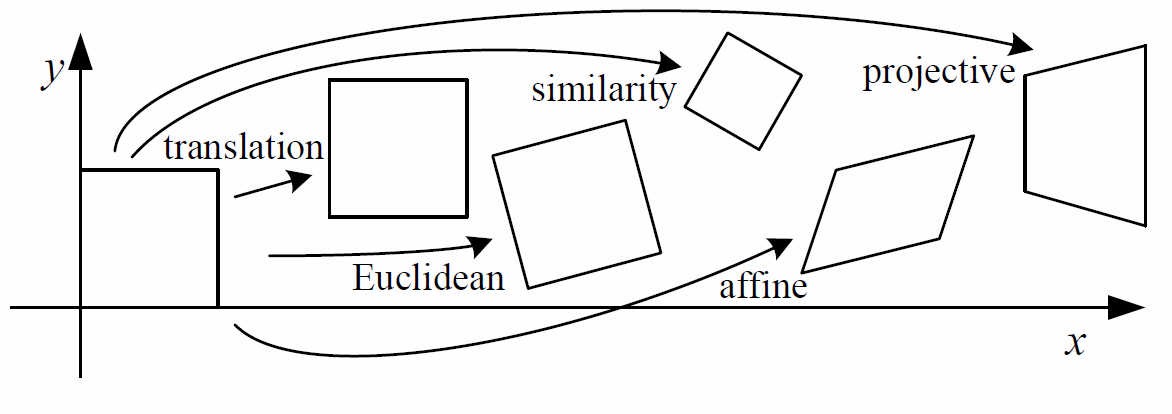
\includegraphics[width=\textwidth]{tweedimensionale_transformaties}
	\caption{Eenvoudige twee-dimensionale transformaties.}
	\label{fig:tweedimensionale_transformaties}
\end{figure}
Elke transformatie maakt gebruik van één of andere matrix. 
\subsection{Similariteit Transformatie}
Deze transformatie combineert eigenlijk de rotatie, translatie en schaling met:
\begin{itemize}
	\item een schalingsfactor $s$,
	\item de rotatiehoek $\theta$,
	\item en deranslatie $t_x$ en $t_y$.
\end{itemize}
$$\begin{bmatrix}
x' \\ y' \\ 1
\end{bmatrix}
=
\begin{bmatrix}
s\cos\theta & -s\sin\theta & t_x \\
s\sin\theta & s\cos\theta & t_y \\
0 & 0 & 1
\end{bmatrix}
\begin{bmatrix}
x \\ y \\ 1
\end{bmatrix}$$

\subsection{Affiene transformatie}
Deze transformatie laat toe om een figuur scheef te maken terwijl parallellisme bewaart blijft.
$$\begin{bmatrix}
x' \\ y' \\ 1
\end{bmatrix}
=
\begin{bmatrix}
a & b & t_x \\
c & d & t_y \\
0 & 0 & 1
\end{bmatrix}
\begin{bmatrix}
x \\ y \\ 1
\end{bmatrix}$$

\subsection{Projectieve transformatie}

$$\begin{pmatrix}
kx' \\ ky' \\ k
\end{pmatrix}
=
\begin{pmatrix}
h_{11} & h_{12} & h_{13} \\
h_{21} & h_{22} & h_{23} \\
h_{31} & h_{32} & h_{33}
\end{pmatrix}
\begin{pmatrix}
x \\ y \\ 1
\end{pmatrix}$$

\section{Drie-dimensionale transformaties}
Tabel \ref{table:DrieDimensionaleTransformaties} toont de hiërarchie van drie-dimensionale transformaties.
\begin{table}
	\centering
	\begin{tabular}{l l c l }
		Transformatie & Matrix & Degrees of Freedom & Behoudt \\
		\hline
		Translatie & $[ I | t]_{3 \times 4}$ & 3 & Oriëntatie \\
		Rotatie & $[ I | t]_{3 \times 4}$ & 6 & Lengte \\
		Similariteit & $[ sR | t]_{3 \times 4}$ & 6 & Hoeken \\
		Affien & $[ A ]_{3 \times 4}$ & 12 & Parallellisme \\
		Projectie & $[ \widetilde{H} ]_{4 \times 4}$ & 15 & Rechte lijnen \\
	\end{tabular}
	\caption{Hiërarchie van drie-dimensionale transformaties.}
	\label{table:DrieDimensionaleTransformaties}
\end{table}
\subsection{Drie-dimensionale rotatie}
\begin{itemize}
	\item Elke rotatie in drie dimensies is rond een as $\textbf{\hat{n}}$
	\item Een verzameling van rotaties rond verschillende assen kan vervangen worden door één rotatie rond één as.
	\item Rotaties in drie dimensies is \underline{niet commutatief}.
	\item Stel:
	$$[\textbf{\hat{n}}]_\times = \begin{bmatrix}
		0 & -\hat{n}_z & \hat{n}_y \\
		\hat{n}_z & 0 & - \hat{n}_x \\
		-\hat{n}_y & \hat{n}_x & 0
	\end{bmatrix}$$
	dan kan elk kruisproduct $\textbf{\hat{n}} \times \textbf{v}$ geschreven worden als
	$$\textbf{\hat{n}} \times \textbf{v} = [\textbf{\hat{n}}]_\times \textbf{v}$$
	\item De rotatiematrix rond een as $\textbf{\hat{n}}$ en hoek $theta$:
	
	$$R(\textbf{\hat{n}}, \theta) = \textbf{I} + \sin \theta [\textbf{\hat{n}}]_\times + (1 - \cos \theta) [\textbf{\hat{n}}]_\times^2$$ 
	Dit staat bekend als de \textbf{formule van Rodrigues}.
	\item Elke beweging van een camera kan geschreven worden als de combinatie van een rotatie met rotatiematrix $\textbf{R}$ en een translatie met translatiematrix $T$: 
	$$
	\begin{bmatrix}
	X_C \\ Y_C \\ Z_C \\ 1
	\end{bmatrix}
	= 
	\begin{bmatrix}
	\textbf{R} & \textbf{T} \\ 0 & 1
	\end{bmatrix}
	\begin{bmatrix}
	X_W \\ Y_W \\ Z_W \\ 1
	\end{bmatrix}
	$$
\end{itemize}

\section{Pinhole model}
\begin{figure}[h]
	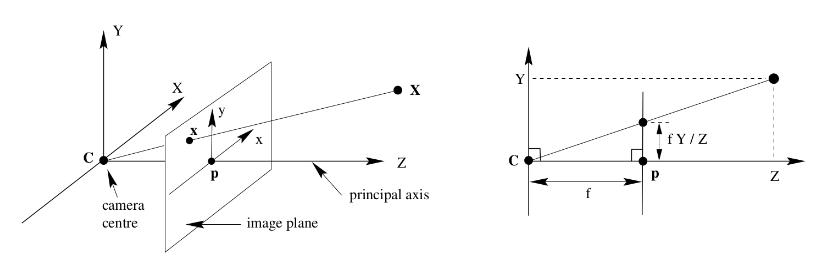
\includegraphics[width=\textwidth]{pinhole_model}
	\caption{Het pinhole model, uitgewerkt voor de yz-vlak.}
	\label{fig:pinhole_model}
\end{figure}
\begin{itemize}
	\item Er wordt een oogpunt $C$ verondersteld.
	\item Op een afstand $f$ bevindt er zicht een projectievlak $p$. 
	Op een lengte $Z$ en hoogte $Y$ bevindt er zich een punt in drie dimensies (analoog voor het xz-vlak, maar dan met lengte $Z$ en hoogte $X$).
	\item Dit driedimensionaal punt kan op het projectievlak geprojecteerd worden door $y = f\frac{Y}{Z}$ en $x = f\frac{X}{Z}$.
	\item Als we nu rekening houden met homogene coördinaten:
	
	$$Z\textbf{x} = Z\begin{pmatrix}
	x \\ y \\ 1
	\end{pmatrix}
	=
	\begin{pmatrix}
	f & 0 & 0 & 0 \\
	0 & f & 0 & 0 \\
	0 & 0 & 1 & 0
	\end{pmatrix}
	\begin{pmatrix}
	X \\ Y \\ Z \\ 1
	\end{pmatrix}
	=
	K_f\textbf{X}$$
	
	De deling door $Z$ verdwijnt en de projectie is nu een lineaire transformatie.
\end{itemize}

\section{Projectieve transformaties}
\begin{itemize}
	\item 
\end{itemize}

